% E2: 200 pairs. Angles are 360 * count / 200; clockwise from 90 degrees.
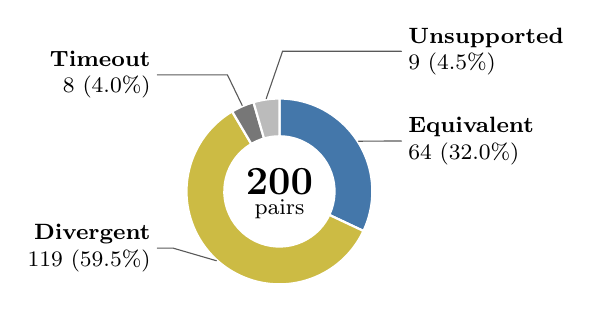
\begin{tikzpicture}[font=\fontsize{8}{9.5}\selectfont, line cap=round]
  \definecolor{eTwoEquivalent}{HTML}{4477AA}
  \definecolor{eTwoDivergent}{HTML}{CCBB44}
  \definecolor{eTwoTimeout}{HTML}{777777}
  \definecolor{eTwoUnsupported}{HTML}{BBBBBB}
  \foreach \start/\finish/\shade in {
    90/-25.2/eTwoEquivalent,
    -25.2/-239.4/eTwoDivergent,
    -239.4/-253.8/eTwoTimeout,
    -253.8/-270/eTwoUnsupported}{
    \path[fill=\shade, draw=white, line width=0.8pt]
      (\start:1.18) arc[start angle=\start,end angle=\finish,radius=1.18]
      -- (\finish:0.70) arc[start angle=\finish,end angle=\start,radius=0.70]
      -- cycle;
  }
  \node[font=\fontsize{15}{16}\selectfont\bfseries] at (0,0.12) {200};
  \node at (0,-0.23) {pairs};

  \draw[black!65, thin] (32.4:1.19) -- (1.36,0.64) -- (1.55,0.64);
  \node[anchor=west,align=left,inner sep=0pt] at (1.63,0.64)
    {\textbf{Equivalent}\\64 (32.0\%)};
  \draw[black!65, thin] (-132.3:1.19) -- (-1.35,-0.72) -- (-1.55,-0.72);
  \node[anchor=east,align=right,inner sep=0pt] at (-1.63,-0.72)
    {\textbf{Divergent}\\119 (59.5\%)};

  \draw[black!65, thin] (113.4:1.19) -- (-0.66,1.48) -- (-1.55,1.48);
  \node[anchor=east,align=right,inner sep=0pt] at (-1.63,1.48)
    {\textbf{Timeout}\\8 (4.0\%)};
  \draw[black!65, thin] (98.1:1.19) -- (0.04,1.78) -- (1.55,1.78);
  \node[anchor=west,align=left,inner sep=0pt] at (1.63,1.78)
    {\textbf{Unsupported}\\9 (4.5\%)};
\end{tikzpicture}
